\documentclass{article}

\usepackage[utf8]{inputenc}
\usepackage[francais]{babel}
\usepackage{amsmath}
\usepackage{amssymb}
\usepackage{fancyhdr}
\pagestyle{fancy}
\usepackage{graphicx}
\usepackage{placeins}
\usepackage{minted}


\lhead{Coralie Saysset - Romain Gerard}
\chead{}
\rhead{B3301}


\begin{document}

\begin{center} 
\Huge{Références croisées \\ Spécification et Conception}
\end{center}



%-----------------------------------------------------------------------------------------------------------------------------------%
%	Spécification compléte
%-----------------------------------------------------------------------------------------------------------------------------------%
\begin{section}{Spécification complète}


  \begin{subsection}{Définitions}

    \begin{itemize}

      \item \textbf{Mot} : Suite de caractères se terminant par un délimiteur

      \item \textbf{Délimiteur} : Un caractère représentant une séparation entre deux mots (Ex: une virgule, un espace, un point, ...) 

      \item \textbf{Ligne} : Suite de mots terminée par un retour chariot

      \item \textbf{Identificateur} : Mot sensible à la casse composé uniquement de caractères alphanumériques et du caractère `\_`. 
				      Un identifacteur commence par une lettre ou par le caractère `\_`.
				      Les commentaires ou chaines litérales ne peuvent contenir d'identifcateurs
				     
      \item \textbf{Mot Clef} : Identificateur que l'utilisateur souhaite rechercher dans un ou plusieurs fichiers. Par défaut il s'agit de ceux du C++

      \item \textbf{Référence croisée} : Fait de rechercher un identificateur dans un ou plusieurs fichiers sources pour déterminer sa localisation
    \end{itemize}

  \end{subsection}


  \begin{subsection}{Description du programme}
    Le but du programme est de permettre de retrouver rapidement l'emplacement d'identifcateurs dans une collection de fichiers.
    L'utilisateur peut choisir de rechercher les identifacateurs étant des mots cléfs, ou ceux qui n'en sont pas.
    On cherche à connaitre dans quel(s) fichier(s) et à quelle(s) ligne(s) ces identifcateurs apparaissent.
    
    Dans le cas où un identifacteur apparaitrait plusieurs fois sur une même ligne, nous avons pris la décision d'afficher
    la ligne concernée autant de fois qu'il y a d'occurences. En effet, un identificateur est un mot clé significatif pour l'utilisateur.
    Nous pouvons donc nous attendre à ce qu'il n'apparaisse que peu de fois sur la même ligne.
    
    Ex: Pour le code ci-dessous présent dans le fichier ``test.cpp'' et avec comme identifacteur la lettre i 
    
    \begin{minted}{cpp}
      for( int i = 0; i < 42; i++ );
    \end{minted}
    Le programme produira la sortie suivante : 

    i$\xrightarrow{}$test.cpp$\bullet$1$\bullet$1$\bullet$1$\downarrow$ \\
    
    Par defaut les mots clefs sont ceux utilisés par le langage C++. Il est cependant possible de spécifier
    un fichier en argument du programme pour définir précisement quels seront les mots clefs recherchés par la référence
    croisée. Le fichier d'identifacteurs ne devra contenir qu'un seul identifacteur valide par ligne, le premier mot de la ligne sera choisi comme tel. Le programme présuposera que
    le fichier fourni en argument respecte ce formalisme.
    
    
  \end{subsection}

  
  \begin{subsection}{Spécifications des options}
    \begin{center}
      \textbf{$tp\_stl\ [-e]\ [-k fichier\_mot\_clef]\ [nomfichier]+$}
    \end{center}

    \begin{itemize}
      \item[] \textbf{-e} : Permet d'inverser le comportement par défaut du programme.
			    Au lieu de rechercher les identificateurs faisant parti du fichier de mot clé, le programme recheche
			    les identificateurs n'étant pas des mots clefs.

      
      \item[] \textbf{-k fichier\_mot\_clef} : Permet de spécifier au programme une liste de mot clé à rechercher par la référence croisée.
					       Par défaut il s'agira des mots-clefs du langage C++ 

      \item[] \textbf{nomfichier} : Chemin vers un ou plusieurs fichiers où rechercher les identifacateurs
    \end{itemize}

  \end{subsection}

\end{section}



%-----------------------------------------------------------------------------------------------------------------------------------%
%	Tests fonctionnels
%-----------------------------------------------------------------------------------------------------------------------------------%
\begin{section}{Tests fonctionnels}

 \begin{subsection}{Méthodologie}
  
    Nous sommes parti du principe que le programme doit produire la même sortie écran (et donc par extension les mêmes données stockées en interne)
    si il est lancé deux fois sur la même collection de fichiers et avec les mêmes arguments.

    En partant de ce principe nous avons réalisé les tests de la façon suivante : 

    \begin{enumerate}
      \item Lancer le programme sur une collection de fichier
      \item Verifier que la sortie est correcte et respecte les spécifications
      \item Relancer le programme dans le même contexte qu'en 1, trier la sortie et rediriger le flux de sortie dans un fichier témoin
    \end{enumerate}

    Pour automatiser les tests nous avons écrit un script bash qui suit les étapes suivantes pour chaque test :
  
    \begin{enumerate}
      \item Lancer le programme dans le même contexte que lors de la réalisation du fichier témoin, trier la sortie et rediriger la sortie vers un fichier résultat
      \item Faire le hash md5 du fichier résultat et du fichier témoin
      \item Comparer les deux hash md5
      \item Si les hashs diffèrent c'est que le programme ne possède pas les mêmes données en interne et donc le test échoue
      \item Si les hashs sont égaux c'est que le programme possède les mêmes données et donc le test est réussi
    \end{enumerate}

 \end{subsection}




 \begin{subsection}{Critique de la méthode}
    \begin{paragraph}{Avantages :}
      Avec cette méthode de réalisation des tests on s'abstrait de la représentation interne des données. On vérifie uniquement
      que le programme délivre correctement à l'utilisateur les informations voulues. Ainsi tout changement dans la structure de
      données interne n'affectera pas les tests tant que le programme délivre les mêmes informations à l'utilisateur.
      
      De plus la réalisation d'un test supplémentaire se fait facilement et ne prend pas beaucoup de temps par rapport à une analyse
      complète de la structure de données interne.
      
      Nous gardons une sauvegarde du flux de sortie lors d'un état fonctionnel de l'application, de ce fait, le développeur peut 
      comparer visuellement les deux sorties pour trouver plus facilement les éléments divergeants. D'où un gain de temps lors du débuggage. 
    \end{paragraph}

    \begin{paragraph}{Inconvénients :}
      Avec cette méthode, le formatage des informations à l'utilisateur devient un élément critique. Tout changement dans l'affichage des résultats causera
      inevitablement l'échec de tous les tests. Toutefois, il peut être facile de créer un script bash permettant de regénérer les fichiers témoins
      si le développeur est sûr des changements qu'il a effectués.
      
      Si un fichier témoin venait à être corrompu cela entrainerait l'échec du test le mettant en jeu.
    \end{paragraph}
 \end{subsection}

  
\end{section}


\newpage
%-----------------------------------------------------------------------------------------------------------------------------------%
%	Architecture générale
%-----------------------------------------------------------------------------------------------------------------------------------%
\begin{section}{Architecture générale}

  \begin{subsection}{Diagramme de classe du module CmdLine}
    \begin{figure}[htp]
      \begin{center}
	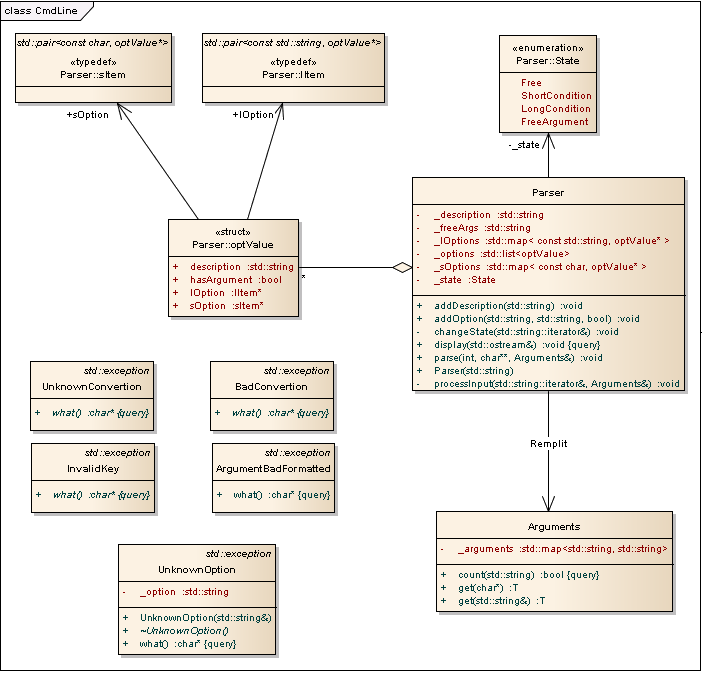
\includegraphics[scale=0.5]{./diagrammeClasse_cmdLine.png}
	% diagrammeClasse.png: 1690x684 pixel, 72dpi, 59.61x24.13 cm, bb=0 0 1690 684
      \end{center}
    \end{figure}
    \FloatBarrier
      Ce diagramme présente les différentes classes présentes pour extraire les informations de la ligne de commande de façon générique.
      
      La classe ``Parser'' s'occupe d'extraire les informations de la ligne de commande en vérifiant que les options entrées par l'utilisateur
      respectent celles définies par le développeur du programme. Au fur et à mesure de l'extraction des données, la classe ``Parser'' remplit
      un objet de la classe ``Arguments''. La classe ``Arguments'' sert de conteneur et permet de convertir les options vers des types déterminés
      à la compilation. Ne sachant pas comment représenter des méthodes génériques en UML, j'ai défini le type de retour des fonctions membres
      ``get'' comme étant T. Le module possède ses propres exceptions pour remonter les cas d'erreurs possibles.
   \end{subsection}
   
   \begin{subsection}{Diagramme de classe du module Reference\_croisée}
    \begin{figure}[!ht]
      \begin{center}
	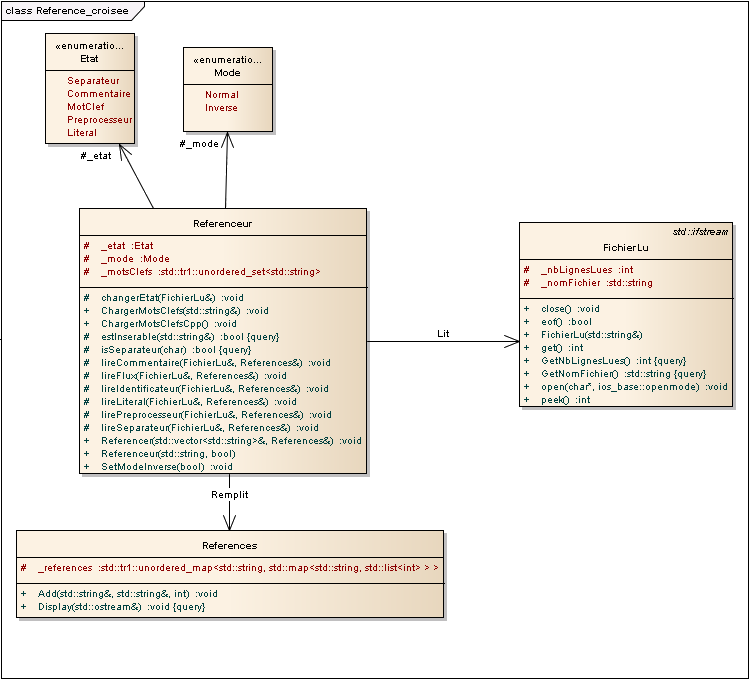
\includegraphics[scale=0.5]{./diagrammeClasse_reference.png}
	% diagrammeClasse.png: 1690x684 pixel, 72dpi, 59.61x24.13 cm, bb=0 0 1690 684
      \end{center}
    \end{figure}
    \FloatBarrier
     Ce diagramme présente les différentes classes utilisées pour extraire les identifacateurs d'un fichier source C++.
      Un objet de la classe ``FichierLu'' permet de lire un fichier stocké sur le disque, tout en fournissant le nombre de lignes déjà 
      lues ainsi que le nom du fichier ouvert. 
      
      Un ``Referenceur'' se sert d'un ``FichierLu'' pour lire les fichiers sources et en extraire les identifacateurs.
      La classe ``References'' permet de stocker les identifacteurs qui sont des mots clefs.
   \end{subsection}
   
   \newpage
    \begin{subsection}{Diagramme de classe du module principal}
    \begin{figure}[!ht]
      \begin{center}
	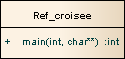
\includegraphics[scale=0.5]{./diagrammeClasse_main.png}
	% diagrammeClasse.png: 1690x684 pixel, 72dpi, 59.61x24.13 cm, bb=0 0 1690 684
      \end{center}
    \end{figure}
    \FloatBarrier
    Le module principal permet d'orchestrer les deux modules précédents pour que le programme ait le comportement attendu.
   \end{subsection}

\end{section}


%-----------------------------------------------------------------------------------------------------------------------------------%
%	Algorithmes principaux
%-----------------------------------------------------------------------------------------------------------------------------------%
\begin{section}{Algorithmes principaux}

  \begin{subsection}{Parseur pour la ligne de commande}
  Pour extraire les informations de la ligne de commande nous utilisons un automate avec un nombre d'états fini.
  
  \begin{paragraph}{Description des états :}
    \begin{itemize}
      \item \textbf{Free} : Lorsque l'automate rencontre quelque chose qui n'est pas un argument ou une option \\Exemple: un caractère séparateur comme un espace
      \item \textbf{ShortCondition} : Lorsque l'automate rencontre une option courte \\Exemple: -e ou -k
      \item \textbf{LongCondition} : Lorsque l'automate rencontre une option longue \\Exemple: - -exclude ou - -keyword
      \item \textbf{FreeArgument} : Lorsque l'automate rencontre un argument rataché à aucune option\\Exemple: le nom d'un fichier à analyser\\
    \end{itemize}
  \end{paragraph}
  
  Une action est déclenché en fonction de l'état de l'automate. L'action extrait, analyse et stocke l'argument de la ligne de commande s'il est valide, sinon une exception est levée.
  \end{subsection}

  \begin{subsection}{Parseur pour les fichiers C++}
  Pour extraire les informations de la ligne de commande nous utilisons ici aussi un automate avec un nombre fini d'états.
  
  \begin{paragraph}{Description des états :}
   \begin{itemize}
    \item \textbf{Separateur} : Lorsque que l'automate rencontre un caractère séparant deux identifacteurs\\Exemple: Tout caractère non alphanumérique, le tiret du bas non inclus
    \item \textbf{Commentaire} : Lorsque l'automate rencontre un commentaire sur une seule ligne ou multiligne \\Exemple: /* Ceci est un commentaire */
    \item \textbf{MotClef} : Lorsque l'automate rencontre un identifacteur qui peut être un mot clef potentiel \\Exemple: cout
    \item \textbf{Preprocesseur} : Lorsque l'automate rencontre une instruction preprocesseur \\Exemple: \#include $<$iostream$>$
    \item \textbf{Literal} : Lorsque l'automate rencontre une chaine de caractères ou un caractère\\Exemple: ``Bonjour''\\
   \end{itemize}
  \end{paragraph}
  
  Chaque état déclenche une action propre qui a pour tâche d'avancer dans le fichier tout en extrayant les identifacteurs recherchés
(ceux qui sont des mots clefs, ou ceux qui n'en sont pas selon l'option choisie).
  \end{subsection}

\end{section}



%-----------------------------------------------------------------------------------------------------------------------------------%
%	Structures de données
%-----------------------------------------------------------------------------------------------------------------------------------%
\begin{section}{Analyse critique des structures de données}


  \begin{subsection}{Structure des mots-clefs}
    \begin {paragraph}{Analyse des besoins :}
    Les mots-clefs sont extraits d'un ou plusieurs fichiers passés en paramètres. À chaque identificateur rencontré durant l'analyse,
    il faut vérifier s'il a déjà été référencé auparavant et si non, créer son entrée dans la structure de données. Le programme devant
    tester de nombreuses fois l'égalité avec un mot clef, nous souhaitons optimiser les accès. De plus chaque mot clef référencé 
    possède une liste de fichiers où il apparait. Il faudra donc pouvoir associer des valeurs aux mots-clefs.
    \end{paragraph}
    
    \begin{paragraph}{Étude d'un arbre binaire :}
     Nous cherchons à optimiser les accès dans la structure de données pour les identificateurs. Dans le pire des cas, si l'arbre
     n'est pas isométrique il faut parcourir tous les noeuds pour savoir si la clef est présente (O(n)). En revanche, dans le cas d'un 
     un arbre équilibré (Ex: un arbre rouge et noir) la recherche est de complexité O(log(n)).
     Un autre avantage d'un arbre binaire est que les mots-clefs seront triés.
     
    \begin{figure}[htp]
    \centering
    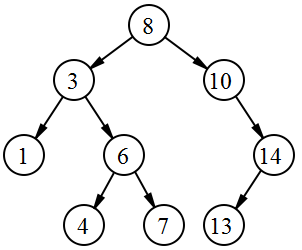
\includegraphics[scale=0.5]{images/arbre.png}
    \caption{Arbre binaire}
    \end{figure}

    \end{paragraph}
    
    \begin{paragraph}{Étude d'une table de hashage :}
     Dans le cas d'une table de hashage l'accès aux données est divisé par une constante C qui est le temps de calcul de la fonction de hashage.
     Nous pouvons dire que l'accès est de compléxité O(1) dans le pire des cas. En contrepartie de cette vitesse d'accès, la table de hashage
     prend plus de place en mémoire que les autres structures de données et les clefs ne sont pas triées. De plus il faut que la fonction de
     hashage soit bien choisit pour qu'il y ait peu de collisions.
     
    \begin{figure}[htp]
    \centering
    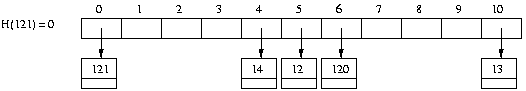
\includegraphics[scale=0.5]{images/hashtable.png}
    \caption{Table de hashage}
    \end{figure}

    \end{paragraph}
    \begin{paragraph}{Decision :}
	Le programme devra fréquement vérifier si un identificateur est un mot clé, donc la structure de donnée doit en priorité favoriser l'accès.
	Notre cahier des charges n'indiquant rien sur une eventuelle limitation de mémoire, on préfèrera utiliser une table de hashage car elle possède la meilleure rapidité d'accès.
    \end{paragraph}

  \end{subsection}

  \begin{subsection}{Structure localisant les Identificateurs}
    \begin{paragraph}{Analyse des besoins :}
    À chaque occurence est associée une paire contenant le nom du fichier et le numéro de ligne où elle apparait, il nous faut donc une structure de données pouvant représenter
    cette multiplicité. Si un mot clef apparait plusieurs fois sur une même ligne nous choisissons de référencer cette ligne autant de fois que le mot clef est présent.
    La compléxité en lecture n'a que peu d'importance dans notre programme car nous devons faire un parcours complet pour afficher toutes les occurences.
    
    Dans un soucis de réutilisabilité, on considère que l'utilisateur pourra en plus de voir apparaître les occurences
    sur la console, vouloir récupérer une structure de données représentant ces occurences.
    \end{paragraph}

    \begin{paragraph}{Étude d'un arbre de liste :}
    Nous pouvons utiliser un arbre de liste pour stocker les occurences des identificateurs. Chaque noeud de l'arbre contient en clef le nom d'un fichier source
    et en valeur la liste des lignes dans lesquelles le mot clef est présent. L'avantage de cette méthode est que nous stockons juste ce qu'il faut, il n'y a pas de redondances
    d'informations. En revanche chaque insertion de référence demandera une complexité moyenne en O(log(n)).
  
    \end{paragraph}
    
    \begin{paragraph}{Étude d'une liste de paire :}
      Chaque occurence étant une paire d'un nom de fichier et d'un numéro de ligne, nous pourrions utiliser une liste pour stocker chacunes de ces paires.
      L'avantage de cette méthode est qu'étant donné que nous lisons les fichiers séquentiellement, l'insertion des paires se fera de manière ordonnée et donc sera de complexité O(1).
      Le désavantage est que nous stockons des doublons, le nom des fichiers où apparaissent les mots clefs.
  
        \begin{figure}[htp]
    \centering
    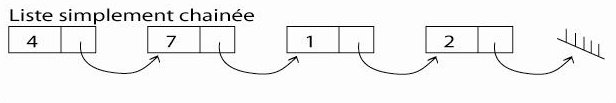
\includegraphics[scale=0.5]{images/liste.jpg}
    \caption{Liste chainée}
    \end{figure}
    \end{paragraph}
      \FloatBarrier

    \begin{paragraph}{Décision :}
      Dans un but de réutilisabilité nous préférons utiliser un arbre de liste pour stocker les références des occurences. Nous évitons la redondance d'informations
      et il sera plus facile de maintenir la cohérence des données si nous souhaitons appliquer des traitements dessus.
    \end{paragraph}
    
  \end{subsection}

\end{section}

\end{document}
